%%%%%%%%%%%%%%%%%%%%%%%%%%%%%%%%%%%%%%%%%%%%%%%%%%%%%%%%%%%%%%%%%%%%%%%%%%%

\documentclass{standalone}

\usepackage{amsmath}
\usepackage{mathptmx}
\usepackage{pgfplots}
\usetikzlibrary{external}
\tikzexternalize{cricket-run-log}
\pgfplotsset{compat=1.16}

%% IEEE uses Times Roman font, so we'll default to Times.
%% These three commands make up the entire times.sty package.
\renewcommand{\rmdefault}{ptm}
\renewcommand{\ttdefault}{pcr}
\normalfont\selectfont

\begin{document}

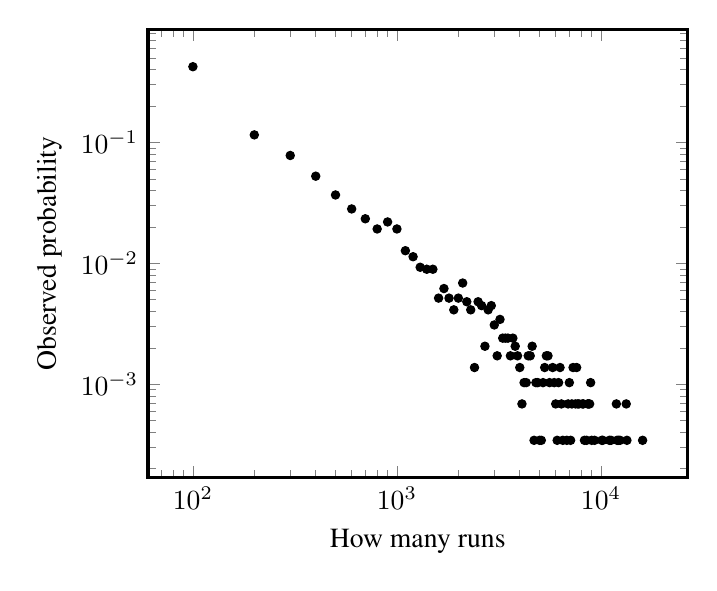
\begin{tikzpicture}
\tikzset{%%
  every mark/.append style={scale=1.0},%%
  scale=1.0%%
}
\pgfplotsset{%%
  every axis/.append style={font=\normalsize}%%
}
%%
\begin{loglogaxis}[%%
  axis line style=very thick,%%
  dotStyle/.style={mark size=1.5,black,mark color=black,mark=*,only marks},%%
  enlargelimits=true,%%
  %% x axis
  xlabel={\normalsize How many runs},%%
  %% y axis
  ylabel={\normalsize Observed probability}%%
]
%%
%%
\addplot[dotStyle] coordinates {
  (100, 0.423024054982818)
  (200, 0.115463917525773)
  (300, 0.078006872852234)
  (400, 0.052577319587629)
  (500, 0.036769759450172)
  (600, 0.028178694158076)
  (700, 0.023367697594502)
  (800, 0.019243986254296)
  (900, 0.021993127147766)
  (1000, 0.019243986254296)
  (1100, 0.012714776632302)
  (1200, 0.011340206185567)
  (1300, 0.009278350515464)
  (1400, 0.00893470790378)
  (1500, 0.00893470790378)
  (1600, 0.005154639175258)
  (1700, 0.006185567010309)
  (1800, 0.005154639175258)
  (1900, 0.004123711340206)
  (2000, 0.005154639175258)
  (2100, 0.006872852233677)
  (2200, 0.004810996563574)
  (2300, 0.004123711340206)
  (2400, 0.001374570446735)
  (2500, 0.004810996563574)
  (2600, 0.00446735395189)
  (2700, 0.002061855670103)
  (2800, 0.004123711340206)
  (2900, 0.00446735395189)
  (3000, 0.003092783505155)
  (3100, 0.001718213058419)
  (3200, 0.003436426116838)
  (3300, 0.002405498281787)
  (3400, 0.002405498281787)
  (3500, 0.002405498281787)
  (3600, 0.001718213058419)
  (3700, 0.002405498281787)
  (3800, 0.002061855670103)
  (3900, 0.001718213058419)
  (4000, 0.001374570446735)
  (4100, 0.000687285223368)
  (4200, 0.001030927835052)
  (4300, 0.001030927835052)
  (4400, 0.001718213058419)
  (4500, 0.001718213058419)
  (4600, 0.002061855670103)
  (4700, 0.000343642611684)
  (4800, 0.001030927835052)
  (4900, 0.001030927835052)
  (5000, 0.000343642611684)
  (5100, 0.000343642611684)
  (5200, 0.001030927835052)
  (5300, 0.001374570446735)
  (5400, 0.001718213058419)
  (5500, 0.001718213058419)
  (5600, 0.001030927835052)
  (5800, 0.001374570446735)
  (5900, 0.001030927835052)
  (6000, 0.000687285223368)
  (6100, 0.000343642611684)
  (6200, 0.001030927835052)
  (6300, 0.001374570446735)
  (6400, 0.000687285223368)
  (6500, 0.000343642611684)
  (6800, 0.000343642611684)
  (6900, 0.000687285223368)
  (7000, 0.001030927835052)
  (7100, 0.000343642611684)
  (7200, 0.000687285223368)
  (7300, 0.001374570446735)
  (7500, 0.000687285223368)
  (7600, 0.001374570446735)
  (7700, 0.000687285223368)
  (7800, 0.000687285223368)
  (8100, 0.000687285223368)
  (8200, 0.000687285223368)
  (8300, 0.000343642611684)
  (8500, 0.000343642611684)
  (8600, 0.000687285223368)
  (8700, 0.000687285223368)
  (8800, 0.000687285223368)
  (8900, 0.001030927835052)
  (9000, 0.000343642611684)
  (9300, 0.000343642611684)
  (10100, 0.000343642611684)
  (10200, 0.000343642611684)
  (11000, 0.000343642611684)
  (11200, 0.000343642611684)
  (11900, 0.000687285223368)
  (12000, 0.000343642611684)
  (12200, 0.000343642611684)
  (12400, 0.000343642611684)
  (13300, 0.000687285223368)
  (13400, 0.000343642611684)
  (16000, 0.000343642611684)
};
\end{loglogaxis}
\end{tikzpicture}

\end{document}
